%+--------------------------------------------------------
%| planar.tex
%|    Specification of planar map
%|
%| by Iddo Hanniel ,Eyal Flato, Dan Halperin, Sariel Har-Peled, 
%| Oren Nechushtan and Shai Hirsch
%+----------------------------------------------------------------------------
%| update log
%|
%| 01 Jun 2000 - Shai Hirsch
%|    Reference parts taken out into planar_ref.tex
%|
%| 03 May 2000 - Shai Hirsch
%|    Transforming to usage of new cc macros.
%|
%| 06 Apr 2000 - Oren Nechushtan
%|    Documentation for the new Planar map (with bounding box).
%|
%| 30 Mar 2000 - Shai Hirsch
%|    Transforming to new format: Separating to User Manual
%|    and Reference Manual. Using new cc commands.
%|    
%| 12 May 2003 - Efi Fogel
%|     Major surgery
%-----------------------------------------------------------------------------

\def\Ipe#1{\def\IPEfile{#1}\input{#1}}

\renewcommand{\Re}{{\rm I\!\hspace{-0.025em} R}}

\def\C{{\cal C}}
\def\G{{\cal G}}
\def\F{{\cal F}}
\def\I{{\cal I}}
\def\U{{\cal U}}
\def\M{{\cal M}}
\def\eps{{\varepsilon}}
\def\bd{{\partial}}
\def\dm{{\cal D}}

\chapter{2D Planar Maps}
\label{I1_ChapterPlanarMap}
\minitoc

\section{Introduction}
\label{PM_sec:intro}

{\em Planar maps} are embeddings of {\em topological maps} into the
plane. A planar map subdivides the plane into vertices, edges, and
faces. The vertices, edges, and faces of a subdivision are the
embeddings of their {\em topological map} counterparts into the plane,
such that (1) each vertex is embedded as a planar point, (2) each edge
is embedded as a bounded $x$-monotone curve, and does not contain
vertices in its interior, and (3) each face is a maximal connected
region of the plane that does not contain edges and vertices in its
interior.

The \ccc{Planar_map_2<Dcel,Traits>} class is derived from the
\ccc{Topological_map<Dcel>} class. While the
\ccc{Topological_map<Dcel>} base class provides the necessary
combinatorial-related capabilities, the
\ccc{Planar_map_2<Dcel,Traits>} class provides all the
geometric-related capabilities required to maintain {\em planar maps}
induced by interior-disjoint $x$-monotone curves, and perform
geometric queries, such as point location.

In this chapter we review the data and functionality added
to the \ccc{Planar_map_2<Dcel,Traits>} class over that of the 
\ccc{Topological_map<Dcel>} class. The combinatorial capabilities of
the base class are covered in chapter ~\ref{I1_ChapterTopologicalMap},
{\em Topological Maps}.

\subsection{Terms and Definitions}
Before we expose a code fragment that manipulates a {\em planar
map}, let us define precisely some of the terms used here after.

\begin{description}
\item[Curve] - the image of a continuous $1$--$1$ mapping into the
plane of any one of the following: the closed unit interval (arc), the
open unit interval (unbounded curve), or the unit circle (closed
curve). In all cases a curve is non self-intersecting. Segments,
lines, rays, conic sections are examples of curves.

\item[{\boldmath $X$}-monotone curve] - a curve that intersects
any vertical line in at most one point, or a vertical segment.

\item[Face] - a maximal connected region of the plane that does not
contain any vertex or edge. We consider a face to be open, and its
boundary is formed by vertices and halfedges of the subdivision.
The halfedges are oriented around a face so that the face they bound 
is to their left. This means that halfedges on the outer boundary
of a face are traversed in counterclockwise order, and halfedges on
the inner boundaries (holes) of a face are traversed in clockwise
order. Halfedges around a vertex are also traversed in clockwise order. 

\item[Point Location] - a query applied to a {\em planar map}. Given a
map and a query point $p$, find the region of the map containing $p$.
\end{description}

\subsection{A simple Program}
The simple program listed below constructs a planar map of three segments

\begin{alltt}
#include <CGAL/Cartesian.h>
#include <CGAL/MP_Float.h>
#include <CGAL/Quotient.h>
#include <CGAL/Pm_segment_traits_2.h>
#include <CGAL/Pm_default_dcel.h>
#include <CGAL/Planar_map_2.h>

typedef CGAL::Quotient<CGAL::MP_Float>    Number_type;
typedef CGAL::Cartesian<Number_type>      Kernel;
typedef CGAL::Pm_segment_traits_2<Kernel> Traits;
typedef Traits::Point_2                   Point_2;
typedef Traits::X_monotone_curve_2        X_monotone_curve_2;
typedef CGAL::Pm_default_dcel<Traits>     Dcel;
typedef CGAL::Planar_map_2<Dcel,Traits>   Planar_map;

int main()
\{
  Planar_map pm;
  X_monotone_curve_2 cv[3];
  Point_2 a1(0,0), a2(0,4), a3(4,0);
 
  cv[0] = X_monotone_curve_2(a1,a2);
  cv[1] = X_monotone_curve_2(a2,a3);
  cv[2] = X_monotone_curve_2(a3,a1);
  pm.insert(&cv[0], &cv[3]);

  return 0;
\}
\end{alltt}

The constructed planar map is instantiated with the
\ccc{Pm_segment_traits_2} traits class to handle segments only. It
consists of two faces, a triangular face and the unbounded face.
This program is not very useful, as it ends immediately after the
planar map is constructed. Let us add something useful, such as
querying whether a point is located in the interior of the single
face of our planar map. All we need to do is issue the following
statements:

\begin{alltt}
  Point_2 p(1,1);
  typedef Planar_map::Locate_type lt;
  (void) pm.locate(p, lt);
  if (lt != Planar_map::FACE)
    std::cout << "Point location failed!" << std::endl;
  else
    std::cout << "Point location passed!" << std::endl;
\end{alltt}

The information returned from the \ccc{locate()} function is
not analyzed further, as this program is presented to illustrates a
simple usage only.

Let us make our simple example a bit more interesting, and draw
the planar map. First, we must add the following include
directives:

\ccInclude{CGAL/IO/Window_stream.h}\\
\ccInclude{CGAL/IO/Pm_Window_stream.h}

Now, we can send the planar map to a window stream after constructing
one, as exemplified in the code fragment below:

\begin{alltt}
  CGAL::Window_stream ws(400, 400);
  ws.init(-0.5, 4.5, -0.5);
  ws << pm;
\end{alltt}

\section{Architecture}
The \ccc{Planar_map_2<Dcel,Traits>} class is parameterized with two
objects. The \ccc{Dcel} object maintains a {\em doubly-connected edge list}
that represents the underlying topological data structure. The
\ccc{Traits} object provides the geometric functionality, and is
tailored to handle a specific family of curves. It encapsulates the
number type used and the coordinate representation. This package
contains traits classes that handle various types of curves (e.g.,
segments, polylines, conics, etc.).

The combinatorial entities have a geometric mapping, e.g.,
a vertex of a planar map has a \ccc{Point} data member and a halfedge
has a \ccc{X_monotone_curve_2} (x-monotone curve) data member.

The \ccc{Planar_map_2<Dcel,Traits>} class consists of a three other
components. (1) It includes a set of interface functions that allow
you to construct, modify, query, save, and restore a planar map,
(2) It is parameterized with a traits concept class that defines the
abstract interface between planar maps and the primitives they use,
and (3) some of its constructors allow you to choose between
various point-location strategies. The point-location strategy has a
significant impact not only on the performance of point-location
queries, but also on the performance of the operations that modify the
planar map.

\subsection{Operations}
The set of operations you can apply to a planar map is divided into
four subsets, namely constructors, modifiers, queries, and
input/output operations. 

\subsubsection{Construction}
A default constructor as well as a copy constructor are
available. However, if you want to override the default point-location
strategy, you must provide the strategy you choose as the single
parameter to the constructor. See section
~\ref{PM_sec:point_location}) for further information.

\subsubsection{Modification}
Once a planar map has been constructed, you can insert an $x$-monotone
curve or a collection of $x$-monotone curves into the map, remove a
curve already in the map, split a curve already in the map into two
curves, and merge two curves already in the map, given that the
resulting curve can be handled by the traits class. All these
operations can be repeated and performed at any order.

Insertion of a collection of $x$-monotone curves into a planar map
that is not empty is not supported yet. However, the aggregate
insertion of a collection of curves into an empty map is drastically
more efficient than the incremental insertion of the curves one at a
time, as the aggregate insertion exploits a dedicated efficient sweep
line algorithm. Notice, that the traits function
\ccc{curves_compare_y_at_x_left()} is not required, nor are the
\ccc{point_reflect_in_x_and_y()} and \ccc{curve_reflect_in_x_and_y()}
functions, if aggregate insertion is the only modification performed
and no queries are performed. 

% Is this true for planar maps, or only for pm with intersections?

% \begin{ccAdvanced}

When additional information detailed below is available, special
insertion function can be used to expedite the insertion of a single
curve. This information may consists of one of the following: (1) the
face containing the curve to be inserted, (2) the vertex containing a
curve endpoint, (3) the two vertices containing the two curve
endpoints respectively, or (4) the halfedges whose incident vertices
contain the curve endpoints respectively. The time complexity of the
insertion operation reduces to $O(1)$, when the incident halfedges are
available and provided to the corresponding special insert function.

The code fragment listed below demonstrates the use of some of the
special insertion-functions.

\begin{alltt}
  Planar_map pm;
  Point_2 a0(0, 0), a1(2, 0), a2(1, 2);

  X_monotone_curve_2 cv[3];
  cv[0] = X_monotone_curve_2(a0, a1);
  cv[1] = X_monotone_curve_2(a1, a2);
  cv[2] = X_monotone_curve_2(a2, a0);

  Planar_map::Halfedge_handle e[3];  
  e[0] = pm.insert_in_face_interior(cv[0], pm.unbounded_face());
  e[1] = pm.insert_from_vertex(cv[1], e[0]);
  e[2] = pm.insert_at_vertices(cv[2], e[1], e[0]->twin());
\end{alltt}

Two halfedges are constructed as a result of inserting a single curve into a
planar map. One of the two new halfedges is returned from the applied function.
The \ccc{insert()} and the \ccc{insert_in_face_interior()} insertion functions
return the new halfedge directed in the same way as the input curve. There are
two flavors of \ccc{insert_from_vertex()} and two falvours of
\ccc{insert_at_vertices()} functions. One accepts vertices and the other
accepts halfedges as additional information to expedite the insertion. These
functions return the new halfedge directed according to the additional
information, regardless of the input-curve direction. The
\ccc{insert_from_vertex()} functions return the new halfedge that has the given
vertex as its source vertex, when a vertex is provided. When a halfedge is
provided instead of a vertex, the target vertex of the given halgedge is the
source of the returned new halfedge. The \ccc{insert_at_vertices()} functions
return the new halfedge, that has the given vertices as its source and target
vertices respectively, when vertices are provided. When halfedges are provided
instead of vertices, the target vertices of the given halgedges are the source
and target of the returned new halfedge respectively.

The next example exploits the most efficient speacial insertion-functions, and
provided to untangle their subtleties. Figure \ref{PM_sec:insert_at} contains
the drawing of the planar map generated by the code fragment listed below.

\begin{figure}[h]
\begin{ccTexOnly}
\centerline{\includegraphics{insert_at.ps}}
\end{ccTexOnly}

\caption{A planar map generated by special insertion functions
\label{PM_sec:insert_at}}

\begin{ccHtmlOnly}
<P>
<center>
  <img src="insert_at.gif"  border=0 alt="insert example output">
</center>
\end{ccHtmlOnly}
\end{figure}

% \ccIncludeExampleCode{Planar_map/example8.C}
\begin{alltt}
  Planar_map pm;
  X_monotone_curve_2 cv1(Point_2(1.0, 0.0), Point_2(3.0, 2.0));
  X_monotone_curve_2 cv2(Point_2(4.0, -1.0), Point_2(3.0, -2.0));
  X_monotone_curve_2 cv3(Point_2(4.0, -1.0), Point_2(1.0, 0.0));
  X_monotone_curve_2 cv4(Point_2(1.0, 0.0), Point_2(4.0, 1.0));
  X_monotone_curve_2 cv5(Point_2(3.0, 2.0), Point_2(4.0, 1.0));
  X_monotone_curve_2 cv6(Point_2(6.0, 0.0), Point_2(4.0, -1.0));
  X_monotone_curve_2 cv7(Point_2(4.0, 1.0), Point_2(6.0, 0.0));

  Halfedge_handle h1 = pm.insert_in_face_interior(cv1, pm.unbounded_face());
  Halfedge_handle h2 = pm.insert_in_face_interior(cv2, pm.unbounded_face());
  Halfedge_handle h3 = pm.insert_at_vertices(cv3, h2->twin(), h1->twin());
  Halfedge_handle h4 = pm.insert_from_vertex(cv4, h1->twin());
  Halfedge_handle h5 = pm.insert_at_vertices(cv5, h1, h4);
  Halfedge_handle h6 = pm.insert_from_vertex(cv6, h3->twin());
  Halfedge_handle h7 = pm.insert_at_vertices(cv7, h5, h6);
\end{alltt}

% \end{ccAdvanced}

\subsubsection{Queries}

In addition to the queries provided by the \ccc{Topological_map<Dcel>}
base class, you can perform point location and vertical ray shoot
queries, and find out whether a given point is contained in a given
face.

The point location and vertical ray-shoot functions, namely
\begin{itemize}
\item
\ccc{Halfedge_handle locate(const Point_2 & p , Locate_type & lt)},
and
\item
\ccc{ Halfedge_handle vertical_ray_shoot(const Point_2 & p, 
                                         Locate_type & lt,
					 bool up_direction )}
\end{itemize}
return the type of the feature that has been located through the
\ccc{Locate_type} reference parameter.

Figure \ref{PM_sec:shoot} contains
the drawing of the planar map generated by example1. This example issues 
a vertical-ray shoot query illustrated in the figure as well. The code of this
program is listed below.

\begin{figure}[h]
\begin{ccTexOnly}
    \centerline{
      \includegraphics{pm_ray_shoot.ps}
    }
\end{ccTexOnly}

\caption{The map generated by example1
\label{PM_sec:shoot}}

\begin{ccHtmlOnly}
    <P>
    <center>
        <img src="example_p.gif"  border=0 alt="example output">
        <!--The map generated by the example program-->
    </center>
\end{ccHtmlOnly}
\end{figure}

The constructed planar map is instantiated with the
\ccc{Pm_segment_traits_2} traits class to handle segments only.
The traits class is instanciated in turn with the \cgal\ Cartesian kernel.
The later is instanciated with the field of quotions of multi-precision
floating-point as the number type. The planar map consists of five segments
that induce three faces. After the construction of the map, its validity
is verified, follwed by a vertical-ray shoot.

\ccIncludeExampleCode{Planar_map/example1.C}

The output of the program is:

\begin{ccExampleCode}
the curves of the map :
1/1 4/1 5/1 7/1
5/1 7/1 9/1 4/1
9/1 4/1 5/1 1/1
5/1 1/1 1/1 4/1
1/1 4/1 9/1 4/1

Inserting the curves to the map ... map valid!

Upward vertical ray shooting from 4/1 3/1
returned the curve 1/1 4/1 9/1 4/1, oriented toward 1/1 4/1
\end{ccExampleCode}

\subsubsection{IO}
The \ccc{Planar Map} package supports saving, restoring, and drawing
of planar maps. Each traits class shipped with this package contains
the necessary I/O operators to save, restore and draw the type of
curves it handles and the type of the curve endpoint.

A simple textual format of a {\em planar map} representation can be
written to the standard output with the \ccc{Extractor} (\ccc{ >> })
operator defined for \ccc{Planar_map_2}. The same format can be read
from the standard input with the \ccc{Inserter} (\ccc{ << }) operator
defined for \ccc{Planar_map_2}. Add the include directive below to
include these operator definitions,

\ccInclude{CGAL/IO/Pm_iostream.h}

Advanced formats, such as XML-based, are currently considered, but
haven't been implemented yet, nor has a binary format.

With the use of the \ccc{Pm_drawer} class a {\em planar map}
representation can be sent to a graphic stream, such as
\ccStyle{leda_window}, Postscript file, or Geomview. Add the include
directive below to include this class definition.

\ccInclude{CGAL/IO/Pm_drawer.h}

Drawing a {\em planar map} with Geomview or producing Postscript that
represents a planar map, can be done by applying the \ccc{Inserter}
operator on the appropriate graphic stream and the planar map
instance. Add the corresponding include directive below, to include
any if these class definitions.

\ccInclude{CGAL/IO/Pm_Postscript_file_stream.h}\\
\ccInclude{CGAL/IO/Pm_Geomview_stream.h}

% Users of I/O functions for the planar map package are required to
% define I/O operators for the curves defined in their \ccc{Traits}
% classes. 

If you intend to save, restore, or draw a planar map, you must
define I/O operators for the point and curve types defined in your
\ccc{Traits} classes, in case these operations are not present. The
traits classes provided in the \ccc{Planar Map} packages, e.g.,
\ccc{Pm_segment_traits_2} and \ccc{Pm_conic_traits_2},
contain the appropriate definitions to save a textual representation
of a planar map to the standard output, restore it from the standard 
input, and draw it to a \cgal\ window stream.

% Are all these provided for polylines?

\begin{ccAdvanced}
\subsection{I/O for User Defined Planar Maps and the I/O Format}

If you wish to add your own attributes planar map components. If
those attributes are to be written as part of the planar map
representation (respectively, are to be re-read later) a specialized
reader (scanner) class (writer class, resp.) should be defined for the
special planar map. This is done preferably by making it a sub class
of the class \ccStyle{Pm_file_scanner} (\ccStyle{Pm_file_writer},
resp.) and overriding all the relevant function for scanning (writing,
resp.) the changed components.

After the definition of the inherited class, you have to call the
function \ccStyle{read} of \ccc{Planar map} (resp., the global
function \ccStyle{write_pm} ) with the inherited class as a
parameter. 

The same applies for extending the output graphic streams to include
additional attributes only for this purpose a new \ccc{drawer}\/ class
has to be defined.  This is done preferably by making this class
inherit the class \ccStyle{Pm_drawer}. In order to send the special
planar map to the graphic stream one should call the global function
\ccStyle{draw_pm} with this class and their planar map as parameters.

\paragraph{Format}
\ccRefLabel{Pm_IO_format}
The chosen format does not follow an existing standard format.
Generally, the format contains lists of the components of a planar map 
followed by each other. For each component we write its associative
geometric information and some topological information in order to be
able to update the \ccc{Dcel} efficiently. The format is detailed
below.

\begin{enumerate}

\item The data begins with a line of three integer values specifying
the number of vertices, halfedges and faces in the planar map.
\item The vertices list: each component in the vertices list contains
the point of its associative vertex. 
\item The halfedges list: each halfedge component is written by an
index indicating the vertex origin of the halfedge, and a curve
specifying the halfedge curve.
\item The faces list: each component in the faces list contains its
outer boundary, if the face is bounded, and a list of its holes which
can be empty in case the face has no holes. The format of the outer
boundary is the number of halfedges of its connected component
followed by the indices indicating the halfedges of that component,
those indices have the same order of the halfedges on the connected
component. The format of the list of the holes is first the number of
holes followed by the connected components per each hole, the format
of each connected components resembles the format of the outer
boundary specified above.
\item Lines beginning with '\#' serve as comments and are ignored.
\item The format does not differentiate between spaces and new lines, 
except new lines which belong to commented lines. 
And hence, writing the planar map in one single line having no comments is
also considered legal. If you would like to keep the commented
lines, they may write all the components between two consecutive
commented lines in one single line.

\end{enumerate}

The current format may not be comfortable for a user to read because
of the extensive use of indices. You can print a planar map in a
verbose format (shorthand for verbose mode format).  The skeleton of 
the verbose format is the same. However, in order for the output to be
clearer for a human reader points and halfedges are explicitly written
rather than being represented by indices. Also the direction of the
halfedges are printed in a more convenient way to read. This verbose
format cannot be scanned by the reading functions of
\ccc{Planar_map_2}.

\ccExample

The example below presents a representation of a planar map containing
one triangle with the coordinates {\em (0,0)}, {\em (1,1)} and {\em
(2,0)}.  The \ccc{Planar_map_2} instance that was used to produce this
example was templated with the \ccStyle{Pm_segment_traits_2}
class, which in turn was templated with the representation class
\ccStyle{Cartesian<leda_rational>}.  The first line specifies that the
planar map has three vertices, six halfedges, and 2 faces (the
triangle and the unbounded face).  The list of vertices each
represented by its associated point follows, as shown in the output
example.  The next list is the one of halfedges, each component is
represented by its index (0,1 or 2) in the vertices list and its
associated segment.  The faces list is presented next. It starts with
the \ccStyle{unbounded face} having one hole which is the triangle,
this connected component specifies that the hole has three halfedges
with the indices 4, 0 and 3. The next face presenting the triangle is
written in the same manner.

\ccIncludeExampleCode{Planar_map/example9.cin}

\subsection{Example of User Defined I/O Functions}
\label{PM_sec:example10}

The following program demonstrates the usage of I/O functions while
users have an additional attribute in their planar map.
The attribute chosen here is adding an associative color to each
vertex. First the program extends the \ccc{Dcel} to maintain this
attribute. Second, the program extends the \ccc{Pm_file_writer} class
to handle the newly defined vertex. 
It simply overrides the functions for writing a vertex to print the
color of the vertex as well. Finally, the main function defines an
empty \ccc{Planar map}, reads it from the standard input stream, and
then set all vertices colors. It then defines an object of its
extended writer class and parameterize the function \ccc{write_pm}
with that object.

\ccIncludeExampleCode{Planar_map/example10.C}

The input of the program is a text file presenting the \ccc{Planar map}:
\ccIncludeExampleCode{Planar_map/example10.cin}

The output is the \ccc{Planar map} written in both formats, non
verbose and verbose. In addition the two lists (non verbose and
verbose) of halfedges are written.
\ccIncludeExampleCode{Planar_map/example10.cout}  

More details are given in sections
\ccc{File_header}\lcTex{
   (\ccRefPage{CGAL::File_header})},
\ccc{Pm_file_scanner<Planar_map>}\lcTex{
   (\ccRefPage{CGAL::Pm_file_scanner<Planar_map>})}, 
\ccc{Pm_file_writer<Planar_map>}\lcTex{ 
   (\ccRefPage{CGAL::Pm_file_writer<Planar_map>})} and
\ccc{Pm_drawer<Planar_map>}\lcTex{
   (\ccRefPage{CGAL::Pm_drawer<Planar_map, Window>})}.

\end{ccAdvanced}

\subsection{Traits Classes}
The planar map class is parameterized with the concept class
\ccStyle{PlanarMapTraits_2} that defines the abstract interface
between planar maps and the primitives they use. It must define two
types of objects, namely \ccStyle{X_monotone_curve_2} and
\ccStyle{Point_2}, where the type of the endpoints of an
\ccStyle{X_monotone_curve_2}-type curve is \ccStyle{Point_2}. In
addition, the traits class must provide a set of operations on these
two types.
					  
We supply a default traits class for segments, namely
\ccStyle{Pm_segment_traits_2<Kernel>}, where \ccStyle{Kernel} is a
kernel representation type, e.g., \ccc{Homogeneous} or
\ccc{Cartesian}. This traits class handles finite line segments in
the plane. In this class the
\ccStyle{X_monotone_curve_2} and \ccStyle{Point_2} types are
defined as the \cgal\ kernel types
\ccStyle{Kernel::Segment_2} and \ccStyle{Kernel::Point_2}
respectively, and the \cgal\ kernel operations on these types are
exploited to implement the required functions.
The \ccc{leda_rat_kernel_traits} class exploits \leda 's rational
kernel and its efficient predicates. As a model that conforms to the
\cgal\ kernel concept, it can be injected to the
\ccStyle{Pm_segment_traits_2<Kernel>} class.
\ccc{leda_rat_kernel_traits} class is available as an external
package.

Models of PlanarMapTraits\_2 are meant to serve as arguments for the
respective template parameter of
\ccc{CGAL::Planar_map_2<Dcel,Traits>}. However, it should be noted
that each model of PlanarMapTraits\_2 defines a family of curves and
primitive geometric operations thereof. Sometimes, the only
implementation available for the manipulation of a certain family of
curves is one of the supplied traits classes. A scenario where one
uses a traits class object to manipulate such curves without
maintaining planar maps is certainly possible.

\ccc{ArrangementTraits_2} concept is a refinements of the
\ccc{PlanarMapWithIntersectionsTraits_2} concept, and the latter is a
refinement of the \ccc{PlanarMapTraits_2} concept.
Therefore, all models of the formers are models of the latter. 
There are several supplied traits classes for the \ccc{Arrangement}
that you can use. These classes are described at the end of Chapter
\ref{I1_ChapterArrangement_2} (\ccc{2D Arrangements}).

\subsection{Point Location Strategies}
\label{PM_sec:point_location}
Some of the basic operations on planar maps are queries such as ``what
is the location of a point in the map?'', or ``which curve is
vertically above the point?''. The answer to these geometric queries can
be obtained through the use of the Planar Map package, along with several
algorithms available for you to choose from.

The \ccClassTemplateName\ class has a point location function
(namely, the \ccc{locate} function that determines which feature of the map 
contains a given query point)
which is also used internally in the \ccc{insert} function.
You can define which algorithm to use in the
point location queries. This is done with a {\em point location class}
passed to the map in the constructor. The class passed should be derived
from the base class \ccc{Pm_point_location_base} which is a
(\ccc{pure virtual}) base class that defines the interface between the 
algorithm implemented by the users and the planar map. This follows the 
known {\it Strategy}
pattern ~\cite{ghjv-dpero-95}. The indirection overhead due to the virtual
functions is negligible since the optimal point location algorithm 
(e.g., the one implemented in our default strategy) takes $\Theta(\log n)$ time.
We have derived three concrete classes for point location strategies,
the {\it default\/} strategy, based on trapezoidal decomposition of the map,
the {\it naive\/} strategy, which goes over all the vertices and halfedges
of the planar map and the {\it walk-along-a-line strategy\/}, which improves
the {\it naive\/} one by ``walking'' only along the zone of the vertical ray
emanating from the query point. All three strategies are classes
that inherit \ccc{Pm_point_location_base<Planar_map>}.
More details are give in sections 
  \ccc{Pm_default_point_location<Planar_map>}\lcTex{
  (\ccRefPage{CGAL::Pm_default_point_location<Planar_map>})}, 
  \ccc{Pm_naive_point_location<Planar_map>}\lcTex{ 
  (\ccRefPage{CGAL::Pm_naive_point_location<Planar_map>})} and
  \ccc{Pm_walk_along_a_line_point_location<Planar_map>}\lcTex{
  (\ccRefPage{CGAL::Pm_walk_along_a_line_point_location<Planar_map>})}.

% If you are an advanced user, you may wish to write your own point
% location class.  We state that a point location class should inherit
% the \cgal\/ supplied class \ccc{Pm_point_location_base<Planar_map>}.

\paragraph{Trade-off Issues}

The main trade-off among the three strategies implemented, is between
time and storage. Using the naive or walk strategies takes more
time but saves storage space.

Another trade-off depends on the need for point location queries compared
to the need for other functions. If you do not need point location 
queries, but do need other modifying functions (e.g., \ccc{remove_edge}, 
\ccc{split_edge} and \ccc{merge_edge}) then using the naive or walk strategies
is preferable. Note that using the \ccc{insert} function invokes the
point location query, therefore when using the naive or walk strategies it
is recommended to use the specialized insertion functions : 
\ccc{insert_in_face_interior}, \ccc{insert_from_vertex} and 
\ccc{insert_at_vertices}.
For example, when using the planar map to represent polygons (e.g., when
computing boolean operations on polygons) it might be preferable to use
the walk strategy with the specialized insertion functions. 

There are two modes of the {\it default\/} strategy which enables
you to choose whether preprocessing should be performed or not (read
more in the section stated above).
There is a trade-off between those two modes. If
preprocessing is not used, the building of the structure is faster. However,
for some input sequences the structure might be unbalanced and therefore 
queries and updates might take longer, especially, if many removal and split 
operation are performed.

\section{Implementation}
\subsection{Robustness}
The \ccc{Planar_map_2<Dcel,Traits>} class can handle all inputs and
requires no general position assumption. Calculations are exact and
leave no place for errors of any kind. Nevertheless, since the input
curves are disjoint in their interiors, no construction of
intersection points are performed. Therefore, filtered kernel can
definitely expedite the various operations.

\subsection{Programming Tips}
This section presents some tips on how to tune
\ccc{CGAL::Planar_map_2<Dcel,Traits>} for best performance.

Before we list specific tips, we remind you that compiling
programs with debug flags turned off, and with optimization flags
turned on, significantly reduces running time.

\begin{enumerate}
   \item The default point location strategy (i.e. using
   \ccc{trapezoidal decomposition}) is the fastest one when queries
   are concerned. However, since it has to build a search structure it
   might slow down the incremental building process of the map. If it
   is known in advance that there will not be many point location or
   vertical ray shoot queries use another point location strategy
   (such as the \ccc{walk} or \ccc{simple} strategies) which does not
   slow down the building process (no search structure is being
   built).

   \item Prior knowledge of the combinatorial structure of the map can
   be used to accelerate insertion time. The specialized insertion
   functions, i.e \ccc{insert_in_face_interior},
   \ccc{insert_from_vertex} or \ccc{insert_at_vertices} should be used
   according to this information. The insert function performs point
   location queries and then calls one of the other update functions
   and therefore takes more time.  The function
   \ccc{insert_in_face_interior} even takes constant time. The other
   two are linear in the worst case, but should be much faster most of
   the time.

   Insertion of a polygon, which is represented by a list of segments
   along its boundary, into an empty planar map should be done in the
   following way. First, some segment should be inserted using
   \ccc{insert_in_face_interior} with the unbounded face. Then a
   segment with a common end point can be inserted using
   \ccc{insert_from_vertex} and so on with the rest of the segments
   but last. The last segment can be inserted using
   \ccc{insert_at_vertices} since both it endpoints are represented as
   vertices of the map and are known in advanced.
 
   \item If you have \leda\/ installed it is recommended to use
   the specialized traits classes \ccc{Pm_leda_segment_traits_2}
   or \ccc{Arr_leda_polyline_traits}. These traits classes are much
   faster since they are specialized for \leda\/'s \ccc{rational
   geometric kernel}. Note that these traits classes are models of
   \ccc{PlanarMapTraits_2} since they model its refinement, the
   \ccc{ArrangementTraits_2} concept.

\end{enumerate}

% \subsection{Performance}

\section{Example Programs}

\subsection{Example of IO functions}
\label{PM_sec:example9}

The following program demonstrates the use of I/O functions provided
for planar maps. 
First the program demonstrates a trivial use of the I/O functions: 
it defines an empty instance of \ccc{Planar_map_2}, 
reads the planar map representation text from the standard input stream, 
and then prints the resulting planar map to the standard output stream.

Second, it presents the usage of the verbose format, 
by defining \ccc{Pm_file_writer} with the verbose flag set to true, 
and then calls the function \ccc{write_pm}.
A usage of the interface of the class \ccc{Pm_file_writer} is also
presented, by calling its function \ccStyle{write_halfedges}, which
prints all the halfedges of the map. In addition, the program presents
the operators writing the resulting  \ccc{Planar map} to a postscript
file when LEDA is installed. The demo for the planar map package makes
use of the output operator of \ccc{Planar_map_2<Dcel,Traits>} to a
window stream  (see at \ccStyle{<CGAL_ROOT>/demo/Planar_map/demo.C} ).   

%graphic streams in commented lines
%(The comments can be removed if you have LEDA installed).

\ccIncludeExampleCode{Planar_map/example9.C}

The input of the program is a text file which holds the planar map
representation in a special format (which is presented in the
reference pages of the the \ccc{Planar Map} package.
This representation appears as the first block in the output file.
 
%\ccIncludeExampleCode{Planar_map/example9.cin}

The output is the \ccc{Planar map} includes both formats, non-verbose
and verbose. In addition the two lists (non-verbose and verbose) of
halfedges are written.
\ccIncludeExampleCode{Planar_map/example9.cout}
